\documentclass{article}

\usepackage[dutch]{babel}
\usepackage{amsmath}
\usepackage{graphicx}

\title{Integration Project}
\author{Kimberly Hengst \emph{1305093}\\ Tim Sonderen \emph{1465252}\\ Kevin Hetterscheid \emph{1490443}\\ Martijn de Bijl \emph{1470108}}
\date{\today}

\begin{document}

\maketitle

\newpage

\section*{Voor gebruik}
\emph{Onze applicatie maakt gebruik van een externe library. Om te code te laten werken, moet deze waarschijnlijk aan de projectpath worden toegevoegd. De jar is al met onze source meegeleverd, dus de instellingen van het project hoeven alleen maar angepast te worden, zodat de jar goed geimporteerd wordt.\\
\phantom{YOLO} \\
Om de applicatie te laten werken moet er een adhoc netwerk opgezet worden, wat alleen in ubuntu kan. Het scriptje adhoc\_setup moet gedraaid worden als root. Ons mulicast adres moet ook toegevoegd worden, dat is 228.5.6.7. }

\newpage

\tableofcontents

\section{Inleiding}
Dit is ons verslag van het project van de derde module. Voor het project hebben wij een chat applicatie gemaakt. In deze applicatie kan een gebruiker in een ad-hoc netwerk met andere gebruikers berichten uitwisselen. De applicatie ondersteunt maximaal vier gebruikers. Een gebruiker kan ervoor kiezen om met \'{e}\'{e}n persoon, of drie andere personen te chatten. De berichten zijn beveiligd met behulp van encryptie. Hierdoor kunnen alleen de andere gebruikers de berichten uitlezen. Als twee gebruikers alleen willen chatten, is dit voor de andere gebruikers ge\"{e}ncrypt.\\
Het netwerk waarop de applicatie draait is een ad-hoc netwerk. Dit betekent dat het netwerk geen router of server nodig heeft. De computers  maken een eigen netwerk via Wi-Fi.
\\
\phantom{YOLO} \\
In het verslag zullen we het proces van het ontwerpen van de applicatie, en de keuzes die we daarbij gemaakt hebben uitleggen. Als eerste bekijken we het ontwerp van de applicatie, hier zal de basis uitgelegd worden. Daarna zal de implementatie van de beveiliging uitgelegd worden. Als laatste zal het test proces beschreven worden.

\newpage

\section{Ontwerp van de applicatie}
De gebruiker kan in een user interface berichten typen en versturen. Deze berichten worden dan in een pakket opgeslagen, en het pakket wordt verstuurd. Het versturen gebeurt via een multicast socket. Dit betekent dat het bericht naar iedereen verstuurd wordt. Als een socket een pakket ontvangt, wordt deze in de GUI weergeven. 

\subsection{Pakketjes}
Voor het versturen van de pakketjes gebruikt multicast socket een Datagram packet. Deze gebruiken wij ook voor het versturen van data. Een datagram packet heeft een byte array met data, een IP adres van de ontvanger, en een poort van de ontvanger. In mulitcast wordt een pakketje dus naar iedereen verstuurd, het IP adres is dan ook het adres van een multicast network, een IP van de IP-klasse D. De poort is een standaard poort waar wij voor hebben gekozen. In de data van de datagram packet worden nog enkele andere velden aangewezen. De eerste byte bevat de sequencenummer, de tweede byte de teller voor het aantal hops, de derde tot zesde byte bestaan uit het IP-adres van de verzender, de zevende tot tiende byte bestaan uit het IP-adres van de ontvanger. We slaan de IP-adressen ook in de header op, omdat het IP-adres in een datagram packet veranderd volgens de context. Bij een ontvangen bericht is het IP-adres die van de verzender, bij een pakket wat verzonden wordt, is het IP-adres die van de ontvanger. \\


\noindent Het pakket ziet er dan als volgt uit:
\\
\begin{tabular}{|c|c|c|c|}
\hline
Byte array data & lengte van data & IP-adres verzender of ontvanger & Poort nummer \\
\hline
\end{tabular}
\\

\noindent Het byte array van de data ziet er dan als volgt uit:
\begin{align*}
\begin{tabular}[center]{| c | c |}
\hline
\multicolumn{2}{|c|}{Byte array data}  \\
\hline
Header & Bericht \\
\hline
\end{tabular}
\end{align*}
\\

De header ziet er dan als volgt uit:
\\
\begin{tabular}{| c | c | c | c | c |}
\hline
\multicolumn{5}{|c|}{Header}  \\
\hline
Sequence nummer & Hop teller & IP-adres verzender & IP-adres ontvanger & Lengte bericht \\
\hline
\end{tabular}
\phantom{YOLO}
\\
\noindent We gebruiken pakketten niet alleen voor het verzenden van berichten uit de GUI, maar ook voor een aantal andere functionaliteiten. De functionaliteiten worden dan in het bericht van de data van het packet toegevoegd. Als het bericht dan met een bepaalde string begint, wordt hiermee een functionaliteit uitgevoerd.
\newpage
De volgende berichten gebruiken wij:
\\

\begin{tabular}{l  p{6cm}l }
Bericht & Functionaliteit \\
\hline
$[FILE]$ & Geeft aan dat het bericht een byte array van een bestand is \\
$[BROADCAST$] & Geeft aan dat het bericht een broadcast is, een bericht dat elke seconde verstuurd wordt om aan te geven dat een persoon er nog is \\
$[NAME\_IN\_USE]$ & Geeft aan dat een naam al in gebruik is, en niet nog een keer gebruikt mag worden \\
$[PRIV\_MESSAGE]$ & Geeft een priv\'{e} bericht aan. Het bericht zal dan alleen aan de ontvanger worden weergeven \\
$[NACK]$ & Geeft aan dat het bericht een NACK is \\
$[TOO\_LATE]$ & Geeft aan dat een bericht waarvoor een NACK is gestuurd niet meer in de buffer voorkomt \\
$[EOF]$ & Geeft het einde van een bestand aan
\end{tabular} \\
\phantom{YOLO} \\
We hebben voor deze header van de pakket gekozen, omdat de methode om het IP-adres van een pakket op de vragen verschilt afhankelijk van de context. Door het IP-adressen in de header weten we zeker dat we de goede adressen hebben. Daarnaast gebruiken we het sequence nummer om te kijken of we alle pakketten hebben binnen gekregen. De hop teller gebruiken we om te zorgen dat pakketjes niet oneindig doorgestuurd worden. Het laatste veld gebruiken we om het bericht goed te ontcijferen. 

\subsection{Bestanden verzenden}
Het verzenden van bestanden gaat ook via Datagram pakketjes. Echter is nu de array van bytes niet een bericht van een gebruiker, maar een deel van een bestand. Bij het versturen wordt een bestand over meerdere pakketjes verdeeld. Dit doen we omdat een bestand niet een pakket zou passen. De verzender kiest een bestand via de GUI die hij wil versturen. Deze wordt dan verzonden, en zodra alle pakketjes bij de ontvanger zijn aangekomen, kan hij deze ergens opslaan. \\


\subsection{Pakket verlies}
Doordat het netwerk via Wi-Fi werkt, en het standaard combinatie met UDP, is de kans dat een pakket verloren gaat veel groter dan via de kabel. Om te zorgen dat deze pakketjes opnieuw worden verstuurd, gebruiken we sequence nummers en NACK's. Als een pakketje verloren gaat, ziet de applicatie dat pas als het volgende pakketje aankomt met een hoger sequence nummer dan verwacht. Als de applicatie een ander sequence nummer binnen krijgt dan verwacht, stuurt de applicatie een negative aknowledgement, een NACK. Omdat er een lange tijd tussen twee berichten kan zitten, bevattem de broadcast berichten ook een sequence nummer, waardoor elke seconde gekeken wordt naar het sequence nummer en het verwachte sequence nummer. \\
We doen het om deze manier, omdat er alleen een bericht gestuurd wordt, als er een bericht mist. Als voor elk pakket een bericht van ontvangst zouden sturen, zou de kans op opstopping groter worden. \\

\subsection{Priv\'{e} chat}
Een gebruiker kan ervoor kiezen om berichten maar naar \'{e}\'{e}n andere gebruiker te sturen. Een gebruiker kan hiervoor kiezen door in de GUI /w en dan de naam van de ontvanger te typen, of op een naam in de lobby te klikken waardoor een priv\'{e} chat begint. Pakketten die alleen voor een bepaalde gebruiker bedoeld zijn worden alleen in zijn GUI weergeven. Andere gebruikers krijgen die pakketten wel binnen, maar ze worden niet standaard uitgelezen. \\

\subsection{User interface}
De gebruiker kan via de user interface met het programma communiceren. De interface bestaat uit een aantal elementen:
\begin{itemize}
\item Tekstveld
\item Typveld
\item Een knop voor het verzenden van tekst en bestanden
\item Een knop voor priv\'{e} chat
\item Een knop voor het afsluiten van het applicatie
\end{itemize}

Via deze interface is het makkelijk met de applicatie communiceren. Alle functionaliteiten kunnen via de interface aangeroepen worden. In het midden is een groot tekst veld, waarin alle berichten verschijnen die gestuurd en ontvangen worden. Daaronder is een tekstveld waarin berichten naar andere gebruikers gestuurd kunnen worden. Aan de linkerkant is een knop voor het versturen van een bestand. Als hierop geklikt wordt, wordt een pop-up geopend waarin een bestand gekozen kan worden. De ontvangers kunnen ervoor kiezen om dit bestand op te slaan of niet, en waar. Ook kan een venster geopend worden voor een persoonlijke chat sessie, door op de naam van een persoon te klikken. Een persoonlijke chat kan ook gevoerd worden in het normale chat venster, door /w "ontvanger" voor het bericht te typen, met als ontvanger de naam van de andere gebruiker.  Er kan voor gekozen worden om persoonlijke berichten in een appart venster te voeren, door de checkbox aan te hebben staan. De applicatie kan afgesloten worden door op de exit knop te drukken.

\section{State diagram}
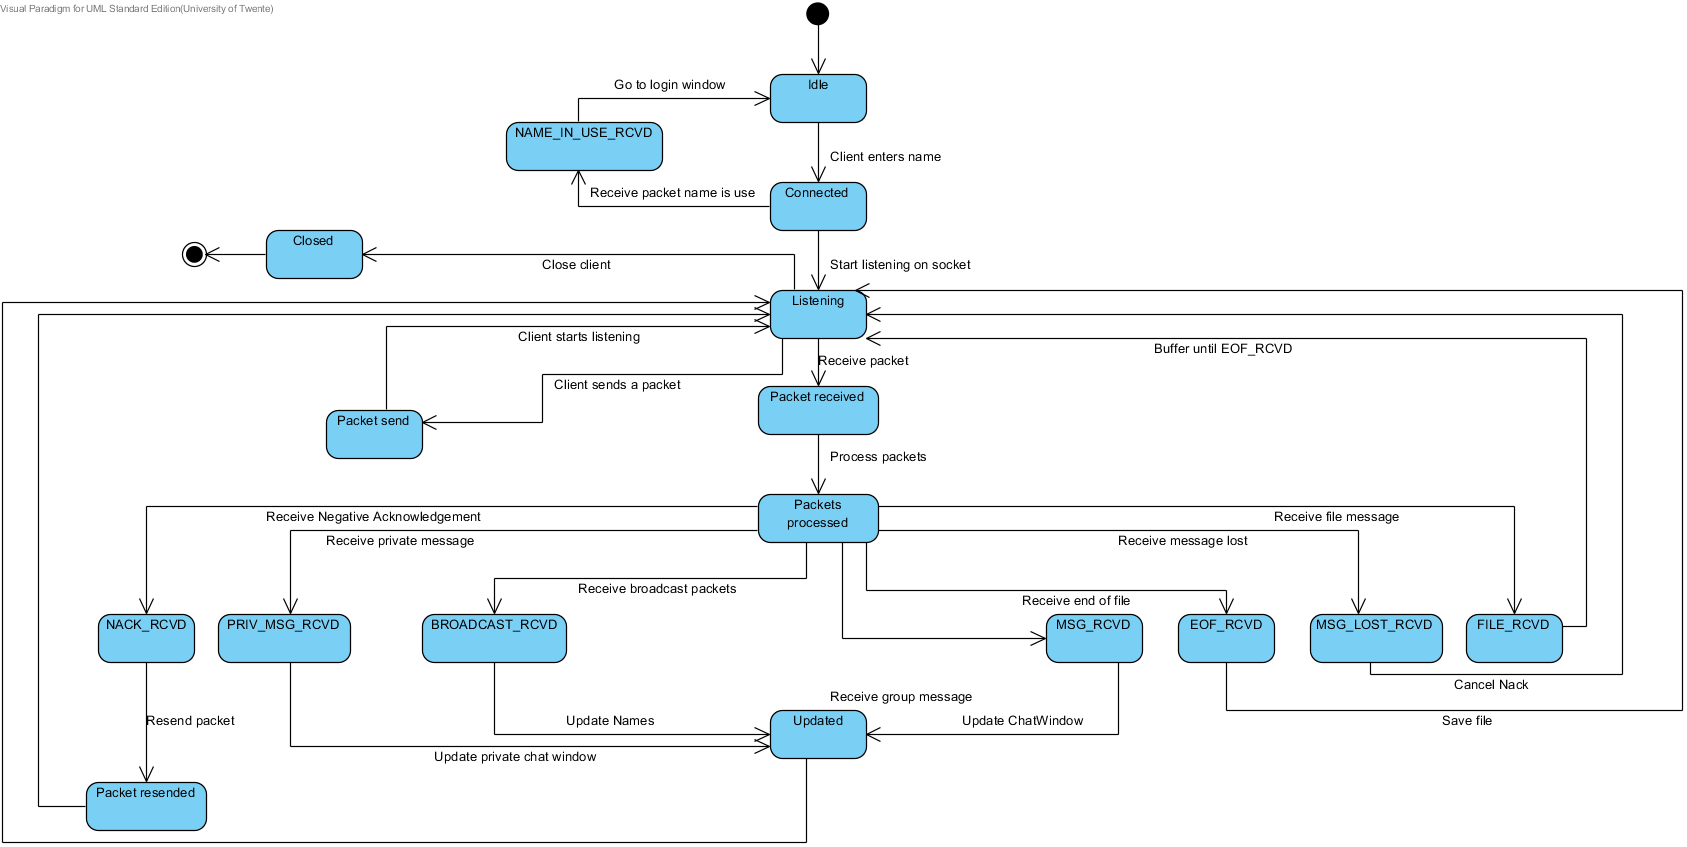
\includegraphics[angle=90, scale=0.6]{chatapplication.png}
\newpage
In het bovenstaande state machine diagram zijn de states te zien die ons programma kan aannemen. We hebben hiervoor de client bekeken. Bij het inloggen is het mogelijk dat er een naam wordt ingevuld die al in gebruik is, hier wordt dan een check voor uitgevoerd, en in het geval dat de naam al in gebruik is, moet de gebruiker een nieuwe naam invullen. \\
Als er een naam is ingevuld die toegestaan is, wordt de gebruiker geconnect in het chatprogramma. De client bevindt zich in een luister staat, die alleen verbroken wordt als hij een pakketje ontvangt. Dan gaat de client naar de staat waarin er pakketjes behandeld worden. Ook kan de luister staat verbroken worden doordat de gebruiker een bericht of een file verstuurd. Dan verzend de client het pakketje. \\
Er zijn een aantal pakketjes die de de client kan ontvangen. Hij kan bijvoorbeeld broadcast pakketjes ontvangen, waarin de naam van de mede chatters wordt mee gestuurd. Hiermee wordt de lijst met namen geupdate, waardoor de gebruiker ook kan zien met wie hij in een chat zit. Ook kan de client pakketjes ontvangen die een bericht bevatten. Dan komt er een prive bericht binnen, of een groepsberichtje. Deze worden dan weergeven op de GUI. Als er een file verzonden wordt door iemand anders, dan ontvangt de client berichtjes waarin dit aangegeven wordt. Ontvangt hij een berichtje dat begint met [FILE], dan weet de client dat dit het begin van een file is. De volgende pakketjes buffert hij, tot hij het berichtje krijgt dat het einde van een file verzending aangeeft. Dit is [EOF]. Als de client een NACK ontvangt, weet hij dat er een ander persoon in de chat is die zijn pakketje niet heeft ontvangen. Het sequence number van het missende pakketje wordt ook in de NACK meegestuurd, waarop de client in zijn buffer van verzonden pakketjes op zoek gaat naar dit desbetreffende pakketje en het opnieuw broadcast. Telkens als de client een pakketje heeft afgehandeld, gaat hij weer naar een luisterstaat. De client is wel in staat meerdere pakketjes tegelijkertijd te ontvangen en te behandelen, doordat de code multithreaded is gemaakt.


\section{Encryptie}
Om te zorgen dat niet iedereen de inhoudt van de pakketten kan lezen, gebruiken we encryptie. Voor de encryptie gebruiken we caesar cipher. Dit betekent dat voor elke byte van de data bij het coderen een vooraf afgesproken getal wordt afgetrokken, en bij het decoderen dat getal er weer bij wordt opgeteld. Dit is geen sterke encryptie, en is makkelijk te kraken met bepaalde algoritmes, maar we hadden geen tijd meer om betere encryptie te implementeren. We waren van plan symetrische AES encryptie te gebruiken. Elke client zou dan een vooraf afgesproken key hebben, waarmee ze zouden kunnen coderen en decoderen. Dit is veel veiliger dan caesar cipher, omdat de data die gecodeerd wordt in blokken gecodeerd wordt. Hierdoor is de key veel lastiger te achter halen. \\

\section{Test plan}
Voor een aantal eisen voor de applicatie hebben we test cases geschreven en uitgevoerd. De volgende eisen hebben we getest:
\begin{itemize}
\item Verzenden berichten
\item Multi-hop
\item Pakket verlies opvangen
\item Beveiliging
\item Bestanden versturen
\end{itemize}

\subsection{Test cases}
\subsubsection{Verzenden berichten \& Pakket verlies}
We verwachten van de applicatie dat elk bericht wat door een gebruiker in de GUI vestuurd wordt, ook verzonden wordt, en aankomt bij de andere gebruikers. Ook moeten verloren pakketten gedecteerd worden, en daarna opnieuw verstuurd worden. \\
Om dit te testen, hebben we een klasse geschreven, die een aantal berichten stuurt. Deze berichten zijn oplopend, bijvoorbeeld 0 tot 99, en worden snel achter elkaar verstuurd. Hierdoor worden een aantal elementen tegelijk getest:
\begin{itemize}
\item Berichten worden verstuurd
\item Berichten komen aan
\item Berichten komen in de goede volgorde aan
\item Pakketverlies wordt gedecteerd
\item Verloren pakketten worden opnieuw verstuurd
\end{itemize}
Daarnaast is er een methode die kijkt hoelang een pakketje erover doet om van een client naar een andere te gaan en weer terug. Deze methode wordt niet alleen be\"{i}nvloed door de tijd over de connectie, maar ook het verwerken van het pakketje. Dit wordt hierin ook in meegenomen. 

\subsubsection{Multi-hop}
We verwachten dat de applicatie berichten doorstuurt die binnen komen. \\
Om dit te testen proberen we ons te verspreiden, zodat twee individuelen nodes elkaars berichten niet meer ontvangen, maar als een node er tussen in gaat staan, die de berichten doorstuurt, de andere twee elkaars berichten weer binnenkrijgt. Doordat de middelste node de berichten doorstuurt. \\
De uitkomst van de test is dat clients die elkaar niet meer kunnen bereiken, elkaar nog wel via een tussenliggende client kunnen bereiken, doordat die de pakketten doorstuurt. In enkele rand gevallen gaat het echter nog niet helemaal perfect, maar dit hebben we uiteindelijk niet meer kunnen oplossen. In de volgende gevallen gaat het fout: \\
\begin{itemize}
\item Als een client een bestand ontvangt, maar halverwege wegloopt, blijft de client wachten op een end of file die niet meer komt.
\item Als een client NACKS heeft gestuurd voor pakket, maar de client waaraan de NACK wordt gestuurd niet meer geconnect is, crasht de applicatie.
\end{itemize}

\subsubsection{Beveiliging}
We verwachten van de applicatie dat de berichten of data uit pakketten versleuteld worden. \\
Dit hebben we getest door naar het netwerk te luisteren met wireshark. Van de pakketjes die we binnen kregen konden we de header uitlezen, maar de data van het pakketjes was onleesbaar. Het is met onze encryptie mogelijk om met een paar pakketjes met data de key te achterhalen, maar dat hebben we niet getest. 

\subsubsection{Bestanden versturen}
We verwachten van de applicatie dat bestanden verstuurd kunenn worden, en indien groter dan wat er in \'{e}\'{e}n pakket past, dat het bestand verdeeld wordt over meerdere pakketten. \\
Om dit te testen, versturen we een aantal bestanden van verschillende groottes. Deze moeten in zijn geheel aankomen. Dit kan gecontroleerd worden door het bestand te openen, en te bekijken of de inhoud nog klopt. Dit is het makkelijkste met plaatjes, omdat hier afwijkingen makkelijker herkent worden. \\
We hebben het oversturen van hele bestanden getest door een groot (\emph{100 Megabytes}) plaatje te sturen. Dit hebben we een aantal keer geprobeerd, en dit ging elke keer goed.\\
We waren van plan om een methode te schrijven die de tijd die het kost om de bestanden te versturen zou meten en uitprinten. Dit is echter niet meer gelukt, en hebben we uiteindelijk geprobeerd om de tijd met de hand te meten. Dit is mogelijk doordat het begin van het versturen van het bestand in de chat verschijnt, en als het bestand helemaal binnen is er een pop-up verschijnt voor het opslaan van het bestand. Dit hebben we verschillende keren gemeten, met verschillende soorten bestanden en groottes. Hiervan hebben we het gemiddelde genomen van bytes per seconde. Het gemiddelde is: 6.3 Megabyte per seconde. 

\end{document}